\documentclass[letterpaper,preprint,11pt]{elsarticle}

\usepackage{graphicx}
\usepackage{graphics} % for pdf, bitmapped graphics files
\usepackage{epsfig} 
\usepackage{multicol}
\usepackage{multirow}
\usepackage{afterpage}
\usepackage{capt-of}
\usepackage{hyperref}
\usepackage{pdflscape}
\usepackage{mathtools}
\DeclarePairedDelimiter\floor{\lfloor}{\rfloor}

\journal{Prof. PR Panda. IIT Delhi}

\begin{document}

\begin{frontmatter}

%% Title, authors and addresses

\title{Minimalistic implementation of lockable Set-associative Cache architecture}

\author{Shreshth Tuli}

\address{Department of Computer Science, IIT Delhi}

\begin{abstract}
%% Text of abstract
This report explains the model and implementation details of lockable Set-Associative cache architectures. When locked, a cache set behaves like a Scratch Pad Memory (SPM). Different features and assumptions for the development of the prototype and testing strategies have also been discussed. The prototype has been developed on VHDL using Xilinx Vivado Design suite.
\end{abstract}
\end{frontmatter}

\section{Model}
The model used to develop the prototype for the Set-Associative Cache is 4 way associative. There is an inherent trade-off between size and speed comparing memroy and cache (given that a larger resource implies greater physical distances) but also a trade-off between expensive, premium technologies (such as SRAM) vs cheaper, easily mass-produced commodities (such as DRAM or hard disks). A 4-way set associative cache looks like the one shown in Fig. \ref{4-set-cache}.


\begin{figure}[h]
\centering
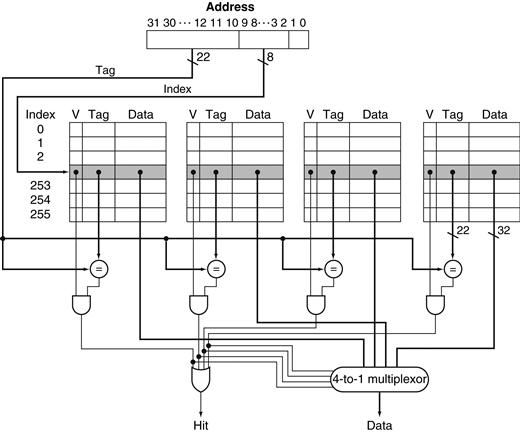
\includegraphics[width=10cm]{4-way-set-cache}
\captionof{figure}{4 way set associative cache}
\label{4-set-cache}
\end{figure}%

\subsection{Design decisions and assumption}
The memory consists of 32 blocks, where each block is of 4 bytes (or 1 word, 32 bits). The cache consists of 4 sets of 2 blocks each. The indexing policy to determine which memory block would be mapped to which set, modulo indexing is used. This means (address \textit{modulo} 4) determines the set number of the corresponding address. Due to this:
\begin{itemize}
\item Address width = $\log_2 32$ = 5
\item Set number [0 to 3] = address \textit{modulo} 4
\item Tag number [0 to 8] = $\floor*{\frac{address}{4}}$
\end{itemize}
The cache design follows write-through policy i.e. whenever data with the some address is present in the cache it is updated both in cache and the memory. The replacement policy used in LRU (Least Recently Used). Each entry also has a tag, which specifies the identity of the data in the backing store of which the entry is a copy. When a cache is locked, a read miss does not lead to replacement of any cache block.
\newline
\newline
The latency of cache read is modeled as 1 clock cycle and that of memory read as 2 clock cycles. For the purpose of ease of development memory write is instantaneous in the model. Memory read/write operations are inherently combinational, 2 cycle delay at the time of memory read is just for modeling purposes.

\section{Implementation}
The model has been implemented using VHDL language and has been simulated using Vivado Design Suite. The source code can be found at the GitHub \href{https://github.com/shreshthtuli/4-Way-set-associative-lockable-cache}{link}.

\section{Simulation and verification}

Fig \ref{sim} shows a simulation of the model generated using Vivado simulation environment. The test signals were generated using VHDL testbench also in the source code.

\subsection{Write testing}
To develop the test a simple testing strategy was used. Initially data was written to addresses 0, 1, 4, 5 in this order. The \textit{rw} signal shown in yellow in the simulation waveform depicts the operation. When \textit{rw} = '0' then data is read from the memory hierarchy and when it is '1', data is written. 

\subsection{Read miss testing}
After writing the data, data is read from the same addresses. As the cache does not have the data corresponding to these addresses, it leads to a miss depicted by \textit{hit} signal which is '0' when miss and '1' when hit occurs. The \textit{hit} signal is shown in white in the simulation waveform. As there is a miss in each case and data needs to be fetched from memory, it shows a \textit{stall} signal (shown in pink) as '1'.

\subsection{Read hit testing}
After reading the data, the cache now is populated with data of addresses 0, 1, 4 and 5. Therefore, reading these data blocks again leads to a cache hit depicted by the \textit{hit} signal and the \textit{stall} signal is also low ('0'). 

\subsection{Lock testing}
Now that the cache is populated, locking a particular cache set should not lead to replacement of blocks in that particular set. When set '0' is locked and set '1' is unlocked, read operations to addresses 8 and 9 lead to miss in both cases. The miss leads to fetching data from the memory and thus \textit{hit} signal is low and \textit{stall} signal is high. Due to locking set '0', the blocks in this set are not replaced and remain 0 and 4, but for set '1' the blocks are overwritten based on LRU policy leading to blocks 5 and 9 (and not 1 and 5). 
 
\begin{landscape}% Landscape page
\begin{figure}[h]
\centering
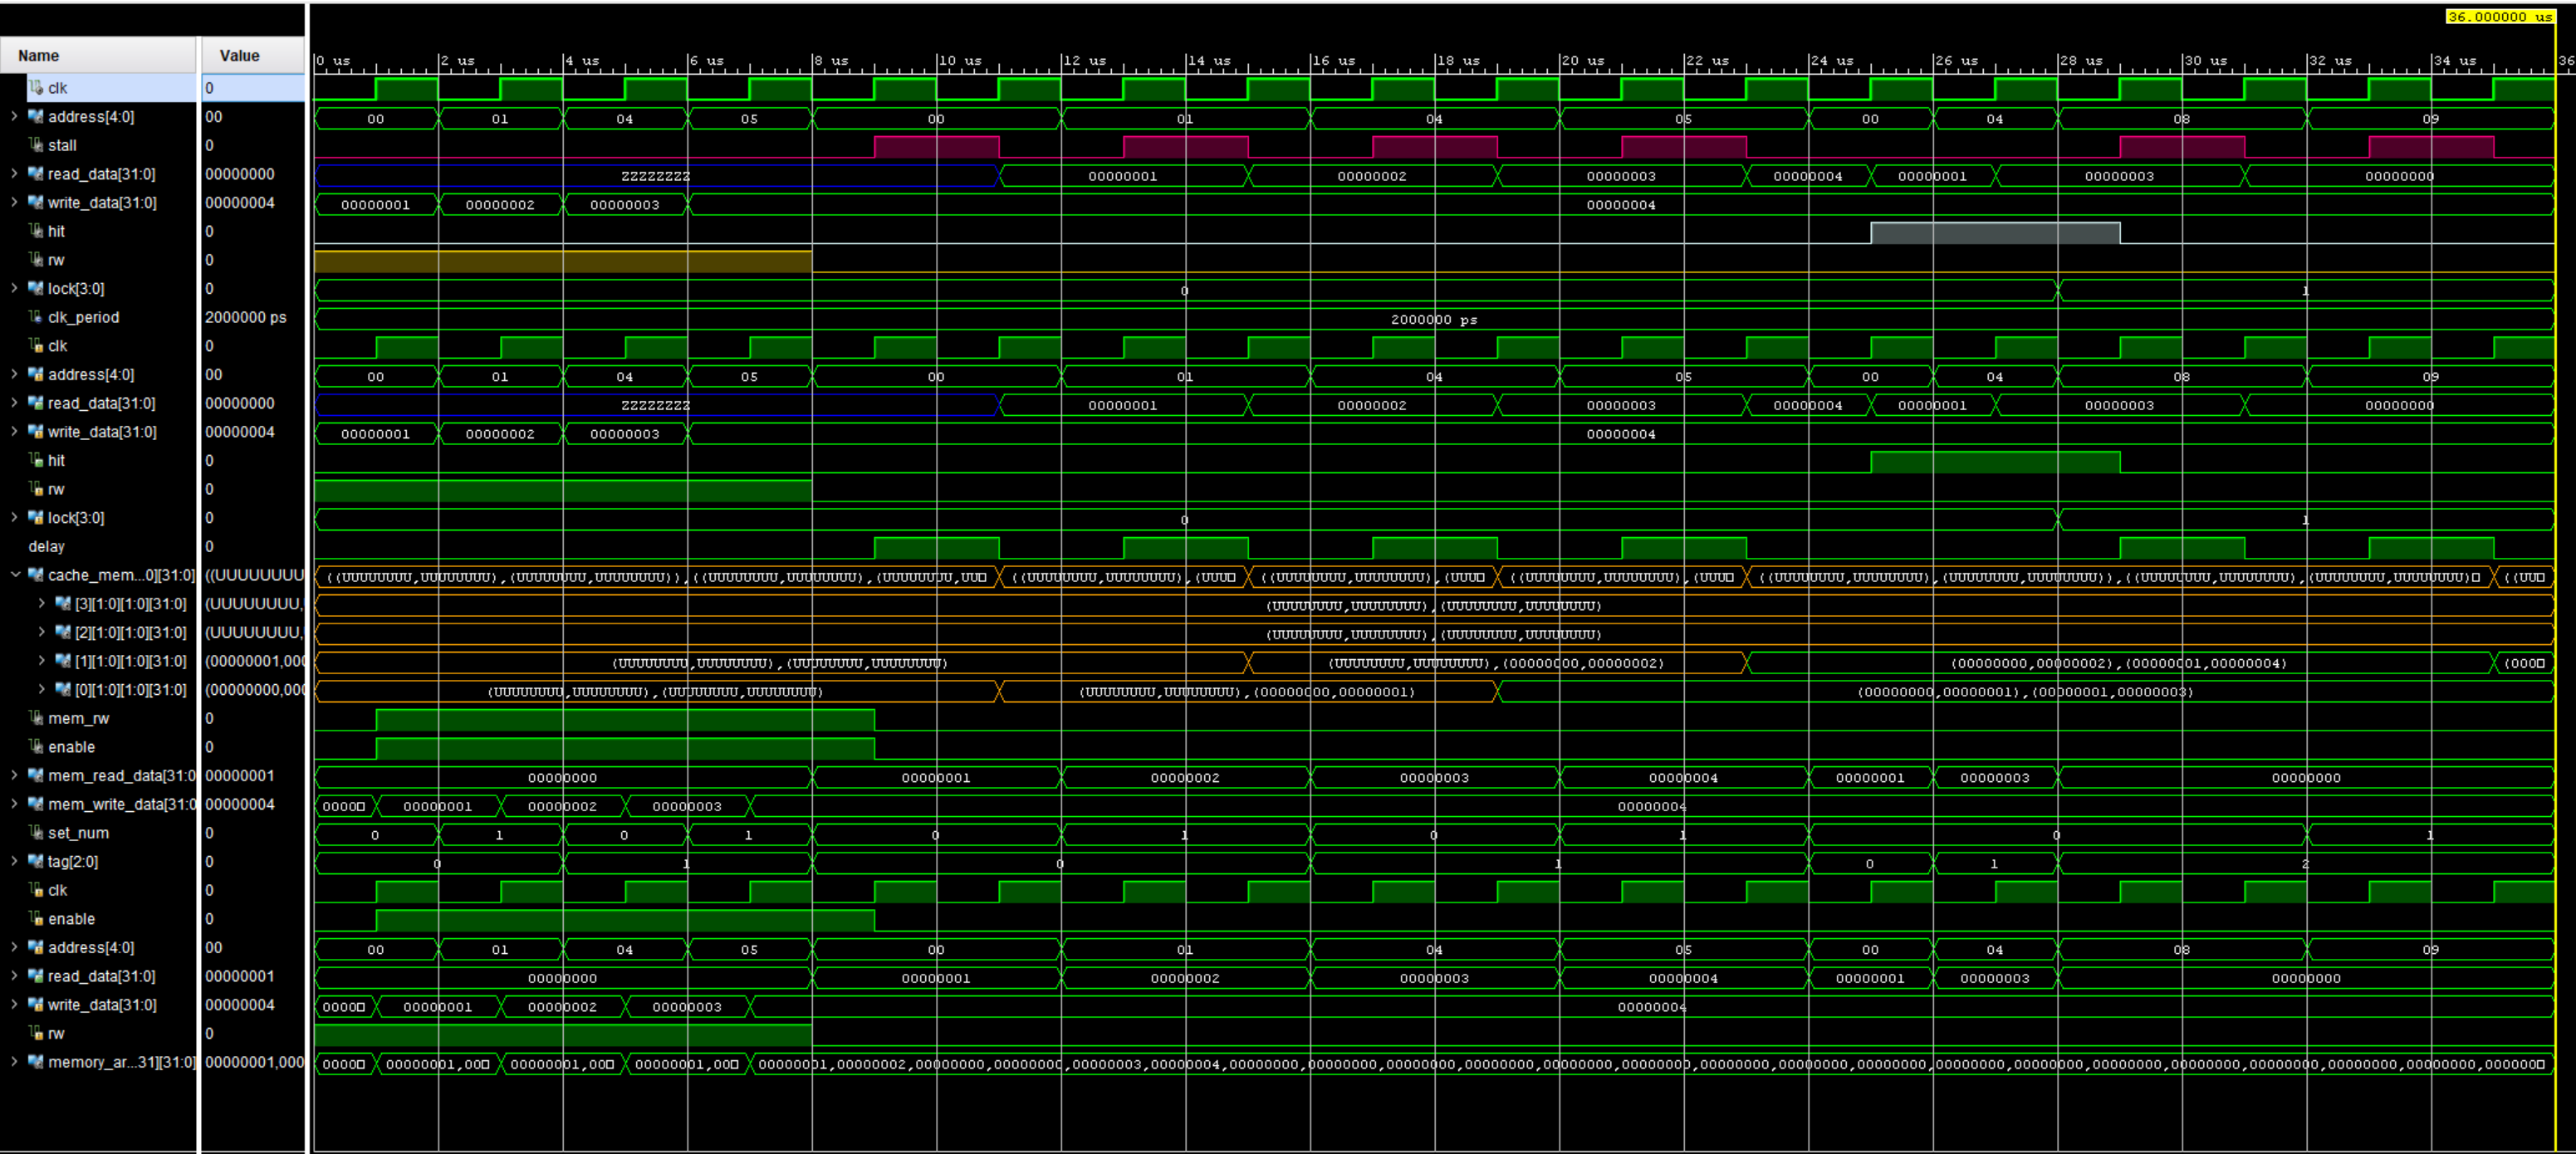
\includegraphics[width=21cm]{Simulation-waveform-colored}
\captionof{figure}{Simulation Waveform}
\label{sim}
\end{figure}%

\end{landscape}

\section{Conclusions}

The prototype developed using VHDL for lockable set-associative cache works well and correctly implements and depicts locking and replacement strategies.






\end{document}
